\chapter{Materiales y M\'etodos}\label{chapter:materials_and_methods}

Para abordar los objetivos establecidos en la introducción, se emplearon los siguientes materiales y métodos.

\section{Datos}

Se emplearon los datos analizados en el estudio [\cite{broderick_mapping_2022}], donde se lleva a cabo un experimento con la participación de 12 sujetos. El objetivo principal de este experimento fue explicar la relación existente entre la frecuencia espacial y la excentricidad en la región V1 del cerebro. Este estudio proporciona una valiosa base de datos, compuesta por estimaciones de amplitud de respuesta de las activaciones neurales, medidas a trav\'es de fMRI, a los diferentes estímulos presentados a los sujetos durante el experimento. Además, se obtuvieron las soluciones de los campos receptivos poblacionales (pRF) de cada sujeto y sus mapas retinot\'opicos.

En esta sección, se brindará una explicación detallada sobre la naturaleza de los datos recopilados en este estudio.

\subsection{Amplitudes de respuesta de la activaci\'on neuronal}

Durante la realización del experimento, se procedió al registro de las respuestas Dependiente del Nivel de Oxígeno en la Sangre (BOLD, por sus siglas en ingl\'es) de los participantes ante un conjunto de est\'imulos de rejilla novedosos. Estos estímulos comprendieron 48 vectores de frecuencia diferentes, distribuidos en 8 fases distintas (0, $\frac{\pi}{4}$, $\frac{\pi}{2}$, ..., $\frac{7\pi}{4}$). Dichos vectores de frecuencia se clasificaron en cinco categorías: angular, radial, espiral hacia adelante, espiral hacia atrás y mixto  (Ver Figura \ref{fig:stim}). Para los primeros cuatro estímulos, se consideraron 10 posibles combinaciones de pares ($\omega_a$,$\omega_r$), donde $\omega_a$ representa la frecuencia angular y $\omega_r$ la frecuencia radial del estímulo, mientras que el último solo abarcó 8 combinaciones posibles (consultar [\cite{broderick_mapping_2022}] para obtener información más detallada). La frecuencia angular $\omega_a$ es un número entero que especifica el número de ciclos de rejilla por revolución alrededor de la imagen, y la frecuencia radial $\omega_r$ especifica el número de radianes por unidad de aumento en $ln(r)$, con $r$ siendo la excentricidad.

\begin{figure}
	\centering
	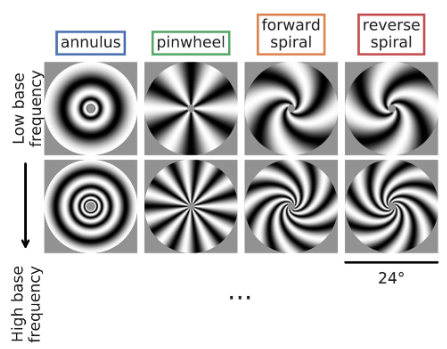
\includegraphics[scale=0.8]{Graphics/stimulus}
	\caption{Ejemplos de est\'imulo angular (annulus), radial (pinwheel), espiral hacia delantes (forward spiral), espiral hacia atr\'as (reverse spiral), utilizados en [\cite{broderick_mapping_2022}]. Tomado de [\cite{broderick_mapping_2022}].}
	\label{fig:stim}
\end{figure}
Las amplitudes de respuesta a estos estímulos, se estimaron utilizando la caja de herramientas \texttt{GLMdenoise} [\cite{kay_glmdenoise_2013}] en el entorno de programación MATLAB. \texttt{GLMdenoise} es una herramienta diseñada para mejorar la calidad de los datos de fMRI, eliminando artefactos y ruido, lo que facilita una interpretación más precisa de la actividad neuronal. El algoritmo ajusta una función de respuesta hemodinámica (HRF, por sus siglas en ingl\'es) específica del observador, estimando las amplitudes de respuesta para cada v\'ertice cortical y cada estímulo mediante 100 ejecuciones de bootstrap. La HRF modela la relación temporal entre la actividad neuronal y los cambios en el flujo sanguíneo en el cerebro.

En consecuencia, se obtuvieron 48 respuestas para cada vóxel (una para cada par único de ($\omega_a$,$\omega_r$)), y estas respuestas fueron promediadas a lo largo de las 8 fases presentadas en las pruebas. Además, el algoritmo incorpora tres regresores polinomiales (grados 0 a 2) para capturar la tendencia media de la señal y la deriva lenta, así como regresores de ruido derivados de vóxeles cerebrales que no se ajustan adecuadamente mediante el modelo lineal general. 

Estos datos se pueden encontrar en \href{https://archive.nyu.edu/handle/2451/63344}{NYU Faculty Digital Archive}.

\subsection{Datos de pRF y mapas retinot\'opicos}

Con el objetivo de obtener información precisa sobre la ubicación y tamaño de los pRF en cada sujeto, se llevó a cabo un experimento de retinotopía independiente. 

Los resultados de este mapeo de pRF se integraron con un atlas retinotópico existente desarrollado por [\cite{benson_retinotopic_2012}], utilizando el método de mapa retinotópico bayesiano propuesto por [\cite{benson_human_2018}]. Este enfoque aprovecha la información detallada de la respuesta de los pRF y la estructura de referencia proporcionada por el atlas retinotópico, lo que permite obtener una representación más precisa y confiable de la organización retinotópica en el cerebro de cada sujeto.

Las estimaciones obtenidas mediante el método bayesiano incluyen la excentricidad, el ángulo polar, el tamaño de los pRF y la delimitación de áreas visuales específicas para cada sujeto. Las áreas visuales estimadas son: V1, V2, V3, hV4, VO1, VO2, LO1, LO2, TO1, TO2, V3b y V3a.

El método bayesiano se llevó a cabo utilizando la biblioteca \texttt{neuropythy} [\cite{benson_human_2018}] de Python, la cual facilita la manipulación y el análisis de datos neurocientíficos. Los datos est\'an disponibles en \href{https://openneuro.org/datasets/ds003812/versions/1.1.0}{OpenNeuro}.


\section{Estimaci\'on de per\'iodo preferido}

En el análisis de los datos mencionados, se empleó la modelación propuesta en [\cite{broderick_mapping_2022}] para ajustar una curva de sintonización log-normal unidimensional a las estimaciones de amplitud de respuesta neural de cada v\'oxel, con el objetivo de estimar los valores de período preferido de estos.

La ecuación del modelo utilizada es la siguiente:
\begin{equation}
\hat{\beta}_b(w_l) = A_b \cdot \exp\left(\frac{-(\log_2(w_l) + \log_2(p_b))^2}{2\sigma_b^2}\right)
\end{equation}
donde \(\hat{\beta}_b(w_l)\) representa la respuesta BOLD promedio en el intervalo de excentricidad \(b\) a la frecuencia espacial \(w_l\) (en ciclos por grado). Los parámetros del modelo incluyen \(A_b\), que es la ganancia de respuesta, \(p_b\), el per\'iodo preferido y \(\sigma_b\), el ancho de banda medido en octavas. El período preferido se define como el recíproco de la frecuencia espacial máxima y se determina como la moda de la curva de sintonización.

La frecuencia espacial local de un est\'imulo visual (\ref{wl}) se define como la norma euclidiana del vector de frecuencia, dividida por la excentricidad  $r$, lo que implica que el período espacial local de los estímulos crece linealmente con la excentricidad [\cite{broderick_mapping_2022}].

\begin{equation}
	w_l(r,\theta) = \dfrac{\sqrt{w_a^2 + w_r^2}}{r} 
	\label{wl}
\end{equation}

Para obtener estimaciones robustas de estos parámetros, se realizaron 100 iteraciones de ajuste por sujeto, por clase de estímulo y por excentricidad, utilizando el método de \textit{bootstrapping}. Este enfoque implicó realizar múltiples ajustes utilizando muestras aleatorias con reemplazo de las 12 ejecuciones de fMRI disponibles (una por cada sujeto).

El método de \textit{bootstrapping} contribuye a la robustez de los resultados al tener en cuenta la variabilidad natural de las respuestas neuronales a lo largo de múltiples repeticiones del experimento. Así, se logra una caracterización detallada de la respuesta de cada v\'oxel, proporcionando información valiosa sobre la frecuencia espacial preferida para diferentes estímulos visuales y en diversas regiones de la excentricidad en el cerebro.

Los m\'odulos necesarios para aplicar esta estimaci\'on, as\'i como las tablas resultantes, se encuentran en el respositorio adjunto a este documento. 

\section{Preprocesamiento de los datos}

En la fase de preprocesamiento, se llevó a cabo una limpieza de los datos para garantizar la confiabilidad y validez de las mediciones. Se tomaron en consideración dos variables de gran importancia en el análisis: la excentricidad y el período preferido de los v\'oxeles.

Se restringi\'o el análisis a v\'oxeles cuya excentricidad se encontraba en un rango entre 1 y 6 grados de \'angulo visual. Esta restricción tiene como objetivo mejorar la fiabilidad de las mediciones, al excluir valores que podrían introducir sesgos o errores en el análisis.

Para los datos de período preferido de los v\'oxeles, se aplicó una transformación logarítmica con el propósito de abordar posibles asimetrías en la distribución de los datos y reducir la escala de los mismos. Además, se llevó a cabo un filtrado al considerar únicamente aquellos valores cuyo logaritmo era mayor que -6. Esta decisión se basa en la necesidad de excluir valores extremadamente pequeños, que podrían afectar la estabilidad numérica del análisis y no aportarían significativamente a la comprensión de la respuesta neuronal. Esta estrategia también contribuye a manejar posibles datos atípicos que podrían influir negativamente en la interpretación de los resultados.

\section{Modelo lineal mixto}
\label{mlm}
Con el objetivo de validar nuestra hipótesis, la cual postula que la frecuencia espacial preferida de los v\'oxeles en el hemisferio derecho es menor que la preferida en el hemisferio izquierdo, hemos implementado un modelo lineal mixto. Este tipo de modelo es una extensión del modelo lineal clásico y permite considerar tanto efectos fijos como aleatorios en los datos. En esta sección, se detallarán los aspectos fundamentales de la formulación de los modelos diseñados para evaluar la hipótesis propuesta. Los resultados obtenidos se encuentran en la Tabla \ref{tab:mlm_results_pp}.

\subsection{Modelo lineal mixto para per\'iodo preferido de v\'ertices corticales}

En la formulación del modelo lineal mixto relacionado con la hip\'otesis, se busca entender la relación entre la frecuencia espacial preferida de los vóxeles y factores como la excentricidad y el hemisferio cerebral. Para ello, utilizando los datos estimados de per\'iodo preferido de los v\'oxeles, se propone el siguiente modelo:

\begin{equation}
	\text{Período Preferido} \sim  \text{Excentricidad} \times \text{Hemisferio} + (1 | \text{Sujeto}) + (1 | \text{Estímulo})	
	\label{mlm_pp}
\end{equation}
donde:
\begin{itemize}
	\item Período Preferido: Representa la variable dependiente que se desea modelar, la cual se define como inverso de la frecuencia espacial preferida.
	
	\item Excentricidad y Hemisferio: Son las variables predictoras que se asocian con el período preferido. La interacción entre la excentricidad y el hemisferio permite capturar las posibles influencias conjuntas de estas variables en la respuesta neuronal.
	
	\item (1 $|$ Subjeto): Este término aleatorio modela la variabilidad entre los diferentes sujetos en el estudio. Cada sujeto puede tener características individuales que contribuyan a la variabilidad en la respuesta neuronal al estímulo visual.

	\item (1 $|$ Est\'imulo): Representa un término aleatorio para cada estímulo utilizado en el experimento. Diferentes estímulos pueden generar respuestas neurales distintas, y este término captura esa variabilidad.
	
\end{itemize}

Este enfoque proporciona una representación completa y realista de la complejidad de los datos observados en el experimento [\cite{broderick_mapping_2022}]. Se empleó el módulo \texttt{lme4} de R para evaluar este modelo y obtener los coeficientes estimados, errores estándar y valores t de las variables fijas, para su análisis.


\subsection{Otros modelos} \label{compare_mlm}

Tambi\'en se comparan varios modelos lineales mixtos para el período preferido. Este enfoque de comparación entre modelos proporciona perspectivas sobre la relevancia de las variables predictoras en la variabilidad del período preferido. A continuación, se formulan y describen los distintos modelos a comparar:

\begin{itemize}
	\item \textbf{Modelo Nulo:}	\\
	Este modelo considera un intercepto constante como único predictor, sin incluir covariables específicas. La variabilidad entre sujetos y estímulos se captura a través de términos aleatorios. Sirve como punto de referencia para evaluar la mejora en la explicación del período preferido al introducir covariables.
	\begin{equation}
		\text{Período Preferido} \sim 1 + (1 | \text{Sujeto}) + (1 | \text{Estímulo})	
		\label{m_1}
	\end{equation}

	\item\textbf{Modelo con Excentricidad:}\\
	En este modelo, se agrega la excentricidad como predictor fijo. Se examina cómo la excentricidad se relaciona con el período preferido, considerando la variabilidad entre sujetos y estímulos. Explora si la excentricidad aporta información significativa sobre el período preferido en comparación con el Modelo Nulo.
	\begin{equation}
		\text{Período Preferido} \sim \text{Excentricidad} + (1 | \text{Sujeto}) + (1 | \text{Estímulo})	
		\label{m_2}
	\end{equation}

	\item \textbf{Modelo Aditivo con Excentricidad y Hemisferio:}\\
	Este modelo incorpora la excentricidad y el hemisferio como predictores fijos. Se busca evaluar cómo ambas variables influyen en el período preferido, considerando la variabilidad entre sujetos y estímulos. Extiende la exploración al agregar el hemisferio como predictor. Permite evaluar la contribución adicional del hemisferio en la explicación del período preferido.
	\begin{equation}
		\text{Período Preferido} \sim \text{Excentricidad} + \text{Hemisferio} + (1 | \text{Sujeto}) + (1 | \text{Estímulo})	
		\label{m_3}
	\end{equation}
	
\end{itemize}

%La comparaci\'on de modelos se realiza utilizando el Criterio de Informaci\'on Bayesiana (BIC, por sus siglas en ingl\'es)\todo{citar}, el cual ayuda a evaluar la calidad de diferentes modelos estadísticos para los mismos datos.  
Para comparar los modelos, se calcula el factor de Bayes. Las comparaciones que se realizan son: el modelo nulo con el modelo con excentricidad, el modelo con excentricidad con el modelo aditivo de excentricidad y hemisferio y la \'ultima comparaci\'on es el modelo aditivo con el modelo \ref{mlm_pp}, al cual se le adiciona la interacci\'on entre las variables fijas.

En el siguiente cap\'itulo se analizan los resultados pertinentes a estas comparaciones.









